\documentclass{book}
\usepackage[landscape,a3paper,left=0.5cm,right=1in,top=1in,bottom=1in]{geometry}
\usepackage{amsmath}
\usepackage{xcolor}
\usepackage{tikz}
\usepackage{pgfplots}
\usepackage{booktabs}
\usepackage{multirow}
\usepackage{amsmath,amssymb}

\begin{document}

\vspace{2cm}

\begin{figure}\caption{\textsc{Equiv + Permut} for Test of 93 small instances of netlib}
\vspace{0.5cm}\centering

\begin{tabular}{cc} & no-solver\\\\\tikz{\node (a) at (0.0,2.5) {\textsc{Algo}};\node (a) at (0.0,0) {};} & 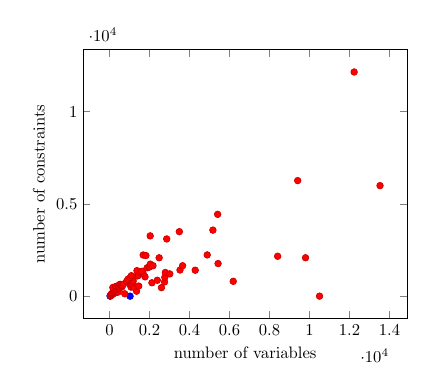
\begin{tikzpicture}[scale=0.6]
\begin{axis}[scatter, point meta=\thisrow{time}, only marks, colorbar, colorbar horizontal,colorbar style={ylabel={Time (min)}, ylabel style={rotate=270},}, colorbar to name={storedcolorbar1},, xlabel=number of variables,ylabel=number of constraints]

\addplot table[x=x,y=y]  { 
 x y time
 33 34 0.05 
 33 34 3.0 
 42 60 2880.0 
 49 71 2880.0 
 98 68 2880.0 
 80 107 2880.0 
 84 116 2880.0 
 104 151 2880.0 
 112 165 2880.0 
 143 164 2880.0 
 141 180 2880.0 
 1027 26 3.0 
 181 159 2880.0 
 163 185 2880.0 
 226 197 2880.0 
 204 250 2880.0 
 283 206 2880.0 
 204 295 2880.0 
 263 264 2880.0 
 309 242 2880.0 
 250 305 2880.0 
 164 495 2880.0 
 302 281 2880.0 
 423 246 2880.0 
 761 155 2880.0 
 316 381 2880.0 
 354 404 2880.0 
 303 545 2880.0 
 481 421 2880.0 
 359 565 2880.0 
 474 446 2880.0 
 458 469 2880.0 
 473 539 2880.0 
 468 566 2880.0 
 10501 27 2880.0 
 615 522 2880.0 
 501 648 2880.0 
 535 666 2880.0 
 588 622 2880.0 
 646 601 2880.0 
 1351 295 2880.0 
 689 673 2880.0 
 1076 516 2880.0 
 1185 520 2880.0 
 1001 682 2880.0 
 855 829 2880.0 
 1076 732 2880.0 
 947 881 2880.0 
 1459 573 2880.0 
 915 937 2880.0 
 1176 821 2880.0 
 1170 863 2880.0 
 1036 1030 2880.0 
 1093 1133 2880.0 
 2595 487 2880.0 
 1377 1117 2880.0 
 2119 749 2880.0 
 1444 1147 2880.0 
 1776 1071 2880.0 
 1372 1405 2880.0 
 1572 1276 2880.0 
 1678 1255 2880.0 
 2388 885 2880.0 
 2751 795 2880.0 
 1621 1373 2880.0 
 2764 1045 2880.0 
 1881 1561 2880.0 
 1989 1598 2880.0 
 2037 1756 2880.0 
 2173 1673 2880.0 
 2790 1306 2880.0 
 3012 1231 2880.0 
 1682 2250 2880.0 
 1819 2221 2880.0 
 3524 1439 2880.0 
 6185 829 2880.0 
 2481 2101 2880.0 
 3653 1671 2880.0 
 4284 1429 2880.0 
 2032 3285 2880.0 
 2858 3119 2880.0 
 5428 1789 2880.0 
 4884 2256 2880.0 
 3490 3512 2880.0 
 8406 2183 2880.0 
 5168 3596 2880.0 
 9800 2103 2880.0 
 5406 4450 2880.0 
 9409 6273 2880.0 
 13526 6001 2880.0 
 12231 12143 2880.0 
};

\end{axis}
\end{tikzpicture}

\\
\tikz{\node (a) at (0.0,2.5) {\textsc{AlgoEnhanced}};\node (a) at (0.0,0) {};} & 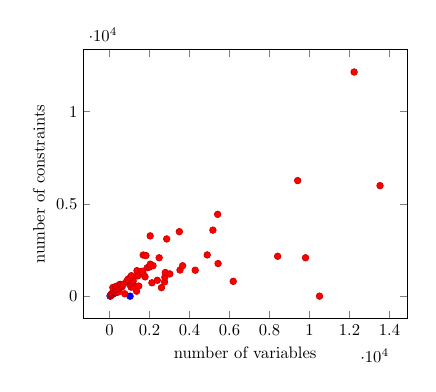
\begin{tikzpicture}[scale=0.6]
\begin{axis}[scatter, point meta=\thisrow{time}, only marks, , xlabel=number of variables,ylabel=number of constraints]

\addplot table[x=x,y=y]  { 
 x y time
 33 34 0.05 
 33 34 0.0 
 42 60 2880.0 
 49 71 2880.0 
 98 68 2880.0 
 80 107 2880.0 
 84 116 133.0 
 104 151 2880.0 
 112 165 2880.0 
 143 164 2880.0 
 141 180 2880.0 
 1027 26 3.0 
 181 159 2880.0 
 163 185 2880.0 
 226 197 2880.0 
 204 250 2880.0 
 283 206 1.0 
 204 295 2880.0 
 263 264 2880.0 
 309 242 2880.0 
 250 305 2880.0 
 164 495 2880.0 
 302 281 2880.0 
 423 246 2880.0 
 761 155 2880.0 
 316 381 2880.0 
 354 404 2880.0 
 303 545 2880.0 
 481 421 2880.0 
 359 565 2880.0 
 474 446 2880.0 
 458 469 2880.0 
 473 539 2880.0 
 468 566 2880.0 
 10501 27 2880.0 
 615 522 2880.0 
 501 648 2880.0 
 535 666 2880.0 
 588 622 2880.0 
 646 601 2880.0 
 1351 295 2880.0 
 689 673 2880.0 
 1076 516 2880.0 
 1185 520 2880.0 
 1001 682 2880.0 
 855 829 2880.0 
 1076 732 2880.0 
 947 881 2880.0 
 1459 573 2880.0 
 915 937 2880.0 
 1176 821 2880.0 
 1170 863 2880.0 
 1036 1030 2880.0 
 1093 1133 2880.0 
 2595 487 2880.0 
 1377 1117 2880.0 
 2119 749 2880.0 
 1444 1147 2880.0 
 1776 1071 2880.0 
 1372 1405 2880.0 
 1572 1276 2880.0 
 1678 1255 2880.0 
 2388 885 2880.0 
 2751 795 2880.0 
 1621 1373 2880.0 
 2764 1045 2880.0 
 1881 1561 2880.0 
 1989 1598 2880.0 
 2037 1756 2880.0 
 2173 1673 2880.0 
 2790 1306 2880.0 
 3012 1231 2880.0 
 1682 2250 2880.0 
 1819 2221 2880.0 
 3524 1439 2880.0 
 6185 829 2880.0 
 2481 2101 2880.0 
 3653 1671 2880.0 
 4284 1429 2880.0 
 2032 3285 2880.0 
 2858 3119 2880.0 
 5428 1789 2880.0 
 4884 2256 2880.0 
 3490 3512 2880.0 
 8406 2183 2880.0 
 5168 3596 2880.0 
 9800 2103 2880.0 
 5406 4450 2880.0 
 9409 6273 2880.0 
 13526 6001 2880.0 
 12231 12143 2880.0 
};

\end{axis}
\end{tikzpicture}

\\
\tikz{\node (a) at (0.0,2.5) {\textsc{LubyTestFullRestart}};\node (a) at (0.0,0) {};} & 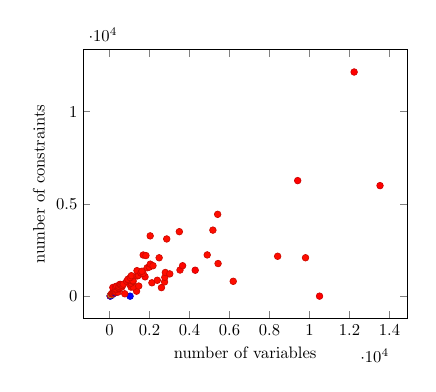
\begin{tikzpicture}[scale=0.6]
\begin{axis}[scatter, point meta=\thisrow{time}, only marks, , xlabel=number of variables,ylabel=number of constraints]

\addplot table[x=x,y=y]  { 
 x y time
 33 34 0.05 
 33 34 0.0 
 42 60 2780.0 
 49 71 2780.0 
 98 68 41.0 
 80 107 580.0 
 84 116 773.0 
 104 151 2783.0 
 112 165 2780.0 
 143 164 2838.0 
 141 180 2780.0 
 1027 26 11.0 
 181 159 2780.0 
 163 185 2780.0 
 226 197 2780.0 
 204 250 2780.0 
 283 206 12.0 
 204 295 2780.0 
 263 264 2780.0 
 309 242 2781.0 
 250 305 2780.0 
 164 495 2851.0 
 302 281 2785.0 
 423 246 2787.0 
 761 155 2780.0 
 316 381 2780.0 
 354 404 2780.0 
 303 545 2801.0 
 481 421 2799.0 
 359 565 2823.0 
 474 446 2880.0 
 458 469 2788.0 
 473 539 2781.0 
 468 566 2780.0 
 10501 27 2880.0 
 615 522 2780.0 
 501 648 2780.0 
 535 666 2880.0 
 588 622 2780.0 
 646 601 2780.0 
 1351 295 2791.0 
 689 673 2780.0 
 1076 516 2780.0 
 1185 520 2780.0 
 1001 682 2786.0 
 855 829 2781.0 
 1076 732 2780.0 
 947 881 2780.0 
 1459 573 2780.0 
 915 937 2799.0 
 1176 821 2780.0 
 1170 863 2786.0 
 1036 1030 2792.0 
 1093 1133 2780.0 
 2595 487 2797.0 
 1377 1117 2780.0 
 2119 749 2782.0 
 1444 1147 2780.0 
 1776 1071 2828.0 
 1372 1405 2791.0 
 1572 1276 2850.0 
 1678 1255 2781.0 
 2388 885 2780.0 
 2751 795 2780.0 
 1621 1373 2787.0 
 2764 1045 2780.0 
 1881 1561 2780.0 
 1989 1598 2782.0 
 2037 1756 2812.0 
 2173 1673 2780.0 
 2790 1306 2780.0 
 3012 1231 2781.0 
 1682 2250 2824.0 
 1819 2221 2784.0 
 3524 1439 2813.0 
 6185 829 2780.0 
 2481 2101 2780.0 
 3653 1671 2834.0 
 4284 1429 2880.0 
 2032 3285 2783.0 
 2858 3119 2780.0 
 5428 1789 2780.0 
 4884 2256 2780.0 
 3490 3512 2780.0 
 8406 2183 2781.0 
 5168 3596 2780.0 
 9800 2103 2780.0 
 5406 4450 2780.0 
 9409 6273 2880.0 
 13526 6001 2880.0 
 12231 12143 2880.0 
};

\end{axis}
\end{tikzpicture}

\\
\\\\
\multicolumn{2}{c}{\ref{storedcolorbar1}}\end{tabular}\end{figure}

\newpage

\begin{figure}\caption{\textsc{Non-Equiv + Permut} for Test of 93 small instances of netlib}
\vspace{0.5cm}\centering

\begin{tabular}{cc} & no-solver\\\\\tikz{\node (a) at (0.0,2.5) {\textsc{Algo}};\node (a) at (0.0,0) {};} & 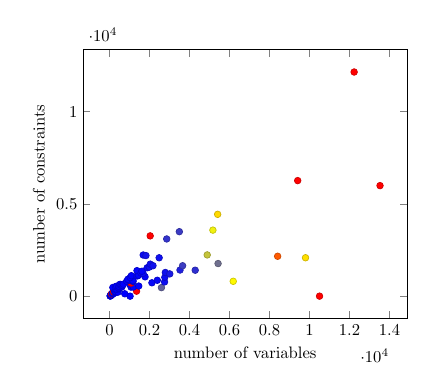
\begin{tikzpicture}[scale=0.6]
\begin{axis}[scatter, point meta=\thisrow{time}, only marks, colorbar, colorbar horizontal,colorbar style={ylabel={Time (min)}, ylabel style={rotate=270},}, colorbar to name={storedcolorbar2},, xlabel=number of variables,ylabel=number of constraints]

\addplot table[x=x,y=y]  { 
 x y time
 33 34 0.05 
 33 34 0.0 
 42 60 0.0 
 49 71 0.0 
 98 68 0.0 
 80 107 0.0 
 84 116 0.0 
 104 151 2880.0 
 112 165 2880.0 
 143 164 0.0 
 141 180 0.0 
 1027 26 3.0 
 181 159 0.0 
 163 185 0.0 
 226 197 0.0 
 204 250 2880.0 
 283 206 0.0 
 204 295 2880.0 
 263 264 0.0 
 309 242 0.0 
 250 305 0.0 
 164 495 0.0 
 302 281 0.0 
 423 246 0.0 
 761 155 1.0 
 316 381 0.0 
 354 404 0.0 
 303 545 0.0 
 481 421 0.0 
 359 565 0.0 
 474 446 0.0 
 458 469 0.0 
 473 539 0.0 
 468 566 0.0 
 10501 27 2880.0 
 615 522 0.0 
 501 648 0.0 
 535 666 1.0 
 588 622 1.0 
 646 601 2.0 
 1351 295 2880.0 
 689 673 1.0 
 1076 516 3.0 
 1185 520 3.0 
 1001 682 4.0 
 855 829 5.0 
 1076 732 2880.0 
 947 881 8.0 
 1459 573 8.0 
 915 937 5.0 
 1176 821 6.0 
 1170 863 6.0 
 1036 1030 7.0 
 1093 1133 7.0 
 2595 487 373.0 
 1377 1117 16.0 
 2119 749 26.0 
 1444 1147 16.0 
 1776 1071 15.0 
 1372 1405 17.0 
 1572 1276 24.0 
 1678 1255 37.0 
 2388 885 31.0 
 2751 795 51.0 
 1621 1373 15.0 
 2764 1045 50.0 
 1881 1561 25.0 
 1989 1598 51.0 
 2037 1756 40.0 
 2173 1673 59.0 
 2790 1306 64.0 
 3012 1231 96.0 
 1682 2250 39.0 
 1819 2221 74.0 
 3524 1439 116.0 
 6185 829 1005.0 
 2481 2101 58.0 
 3653 1671 229.0 
 4284 1429 174.0 
 2032 3285 2880.0 
 2858 3119 191.0 
 5428 1789 422.0 
 4884 2256 737.0 
 3490 3512 220.0 
 8406 2183 2200.0 
 5168 3596 905.0 
 9800 2103 1200.0 
 5406 4450 1241.5 
 9409 6273 2880.0 
 13526 6001 2880.0 
 12231 12143 2880.0 
};

\end{axis}
\end{tikzpicture}

\\
\tikz{\node (a) at (0.0,2.5) {\textsc{AlgoEnhanced}};\node (a) at (0.0,0) {};} & 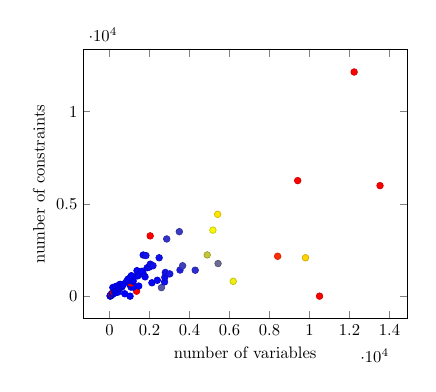
\begin{tikzpicture}[scale=0.6]
\begin{axis}[scatter, point meta=\thisrow{time}, only marks, , xlabel=number of variables,ylabel=number of constraints]

\addplot table[x=x,y=y]  { 
 x y time
 33 34 0.05 
 33 34 0.0 
 42 60 0.0 
 49 71 0.0 
 98 68 0.0 
 80 107 0.0 
 84 116 0.0 
 104 151 2880.0 
 112 165 2880.0 
 143 164 0.0 
 141 180 0.0 
 1027 26 3.0 
 181 159 0.0 
 163 185 0.0 
 226 197 0.0 
 204 250 2880.0 
 283 206 0.0 
 204 295 2880.0 
 263 264 0.0 
 309 242 0.0 
 250 305 0.0 
 164 495 0.0 
 302 281 0.0 
 423 246 0.0 
 761 155 0.0 
 316 381 0.0 
 354 404 0.0 
 303 545 0.0 
 481 421 0.0 
 359 565 0.0 
 474 446 0.0 
 458 469 0.0 
 473 539 0.0 
 468 566 0.0 
 10501 27 2880.0 
 615 522 0.0 
 501 648 0.0 
 535 666 1.0 
 588 622 1.0 
 646 601 2.0 
 1351 295 2880.0 
 689 673 1.0 
 1076 516 3.0 
 1185 520 4.0 
 1001 682 4.0 
 855 829 5.0 
 1076 732 2880.0 
 947 881 6.0 
 1459 573 7.0 
 915 937 5.0 
 1176 821 7.0 
 1170 863 5.0 
 1036 1030 8.0 
 1093 1133 6.0 
 2595 487 325.0 
 1377 1117 12.0 
 2119 749 20.0 
 1444 1147 16.0 
 1776 1071 15.0 
 1372 1405 21.0 
 1572 1276 25.0 
 1678 1255 29.0 
 2388 885 31.0 
 2751 795 53.0 
 1621 1373 15.0 
 2764 1045 49.0 
 1881 1561 25.0 
 1989 1598 51.0 
 2037 1756 37.0 
 2173 1673 61.0 
 2790 1306 64.0 
 3012 1231 94.0 
 1682 2250 39.0 
 1819 2221 72.0 
 3524 1439 113.0 
 6185 829 894.0 
 2481 2101 58.0 
 3653 1671 245.0 
 4284 1429 169.0 
 2032 3285 2880.0 
 2858 3119 193.0 
 5428 1789 409.0 
 4884 2256 742.0 
 3490 3512 225.0 
 8406 2183 2534.0 
 5168 3596 931.0 
 9800 2103 1283.0 
 5406 4450 1150.5 
 9409 6273 2880.0 
 13526 6001 2880.0 
 12231 12143 2880.0 
};

\end{axis}
\end{tikzpicture}

\\
\tikz{\node (a) at (0.0,2.5) {\textsc{LubyTestFullRestart}};\node (a) at (0.0,0) {};} & 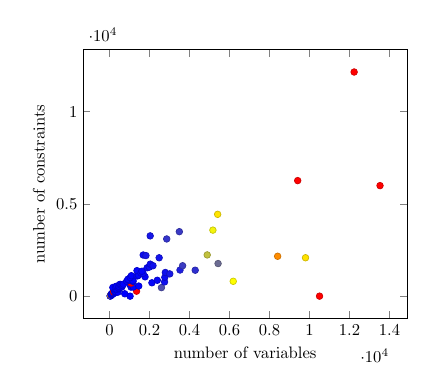
\begin{tikzpicture}[scale=0.6]
\begin{axis}[scatter, point meta=\thisrow{time}, only marks, , xlabel=number of variables,ylabel=number of constraints]

\addplot table[x=x,y=y]  { 
 x y time
 33 34 0.05 
 33 34 0.0 
 42 60 0.0 
 49 71 1440.0 
 98 68 0.0 
 80 107 0.0 
 84 116 0.0 
 104 151 0.0 
 112 165 0.0 
 143 164 0.0 
 141 180 0.0 
 1027 26 3.0 
 181 159 0.0 
 163 185 0.0 
 226 197 0.0 
 204 250 2880.0 
 283 206 0.0 
 204 295 2880.0 
 263 264 0.0 
 309 242 0.0 
 250 305 0.0 
 164 495 0.0 
 302 281 0.0 
 423 246 0.0 
 761 155 1.0 
 316 381 0.0 
 354 404 0.0 
 303 545 0.0 
 481 421 0.0 
 359 565 0.0 
 474 446 0.0 
 458 469 0.0 
 473 539 0.0 
 468 566 0.0 
 10501 27 2880.0 
 615 522 0.0 
 501 648 0.0 
 535 666 1.0 
 588 622 1.0 
 646 601 2.0 
 1351 295 2880.0 
 689 673 1.0 
 1076 516 3.0 
 1185 520 3.0 
 1001 682 4.0 
 855 829 5.0 
 1076 732 2880.0 
 947 881 7.0 
 1459 573 7.0 
 915 937 5.0 
 1176 821 8.0 
 1170 863 5.0 
 1036 1030 6.0 
 1093 1133 7.0 
 2595 487 299.0 
 1377 1117 12.0 
 2119 749 21.0 
 1444 1147 16.0 
 1776 1071 16.0 
 1372 1405 21.0 
 1572 1276 24.0 
 1678 1255 28.0 
 2388 885 31.0 
 2751 795 60.0 
 1621 1373 15.0 
 2764 1045 47.0 
 1881 1561 30.0 
 1989 1598 52.0 
 2037 1756 37.0 
 2173 1673 62.0 
 2790 1306 65.0 
 3012 1231 93.0 
 1682 2250 40.0 
 1819 2221 85.0 
 3524 1439 112.0 
 6185 829 969.0 
 2481 2101 72.0 
 3653 1671 226.0 
 4284 1429 176.0 
 2032 3285 81.0 
 2858 3119 197.0 
 5428 1789 407.0 
 4884 2256 725.0 
 3490 3512 219.0 
 8406 2183 1824.0 
 5168 3596 915.0 
 9800 2103 1177.0 
 5406 4450 1158.0 
 9409 6273 2880.0 
 13526 6001 2880.0 
 12231 12143 2880.0 
};

\end{axis}
\end{tikzpicture}

\\
\\\\
\multicolumn{2}{c}{\ref{storedcolorbar2}}\end{tabular}\end{figure}

\newpage

\end{document}